\section{Discussion}
\label{Discussion}
\textbf{FIXME: La conclusione la incorporo come subsection della discussion o la tengo separata? }\\
In this section we discuss the issues, the results and the possible future development of our generator. We also present a use case to show how the generator works on a simple transformation.

FIXME: Modify the list of topics here:
\begin{itemize}
 \item Acceleo cannot get more than one input file, that means we cannot read the information from the WSDL file(s).
  \subitem The variables types have to be input manually
  \subitem The "assign" activities cannot be translated automatically
  \subitem The infos to invoke a real web service are inside the WSDL file
 \item solutions:
  \subitem Modify Acceleo API, or wait for Acceleo to support this thing.
  \subsubitem We tried to talk with the Acceleo developers but it was not time wise feasible task
  \subitem Un'idea per sormontarli sarebbe di andare a creare un'altra trasformazione Acceleo, che dato in input un file WSDL, scrive le informazioni necessarie in un file Java-properties che verrà poi usato dall'applicazione Java. Se i file WSDL sono più di uno, la trasformazione viene eseguita più volte (a seconda del numero dei file WSDL) andando ad aggiungere altre linee nel file Java-properties
\end{itemize}

\subsection{Use Case}
\label{sec:UseCase}
FIXME, to complete with some pictures. \ref{fig:GeneratorUseCase}
\begin{itemize}
 \item The input model complying with our workflow pattern
 \item Run the Acceleo generation
 \item Create an instance of the Java application process' class and run the runWorkflow() method.
 \item The behaviour is the same as when we run an instance of the BPEL's process 
\end{itemize}

\begin{figure}
  \begin{center}
    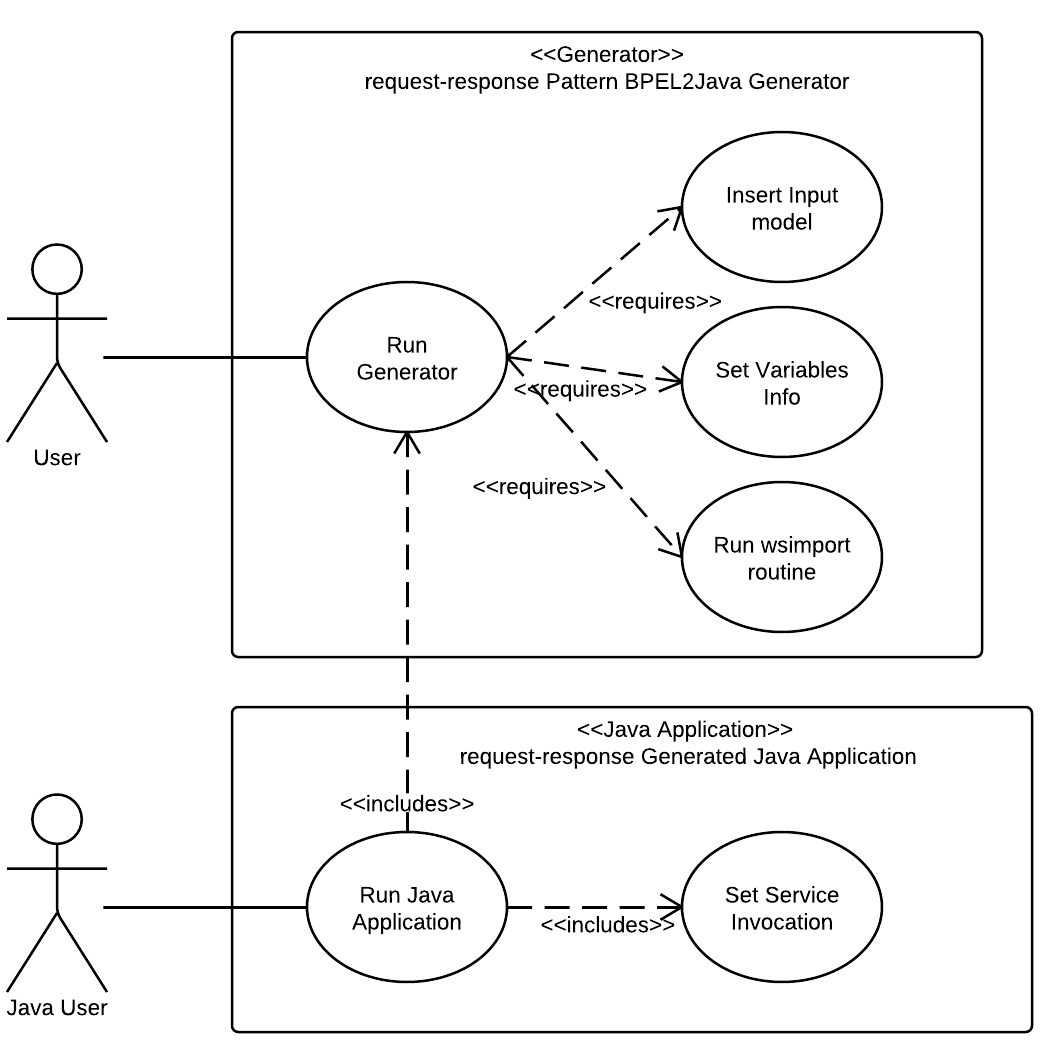
\includegraphics[scale=1.5]{pictures/GeneratorUseCase.png}
    \caption{Use Case}
    \label{fig:GeneratorUseCase}
  \end{center}
\end{figure}



\subsection{Future Development}
\label{sec:FutureDevelopment}

